\documentclass[oneside]{book}

% Packages required by doxygen
\usepackage{fixltx2e}
\usepackage{calc}
\usepackage{doxygen}
\usepackage[export]{adjustbox} % also loads graphicx
\usepackage{graphicx}
\usepackage[utf8]{inputenc}
\usepackage{makeidx}
\usepackage{multicol}
\usepackage{multirow}
\PassOptionsToPackage{warn}{textcomp}
\usepackage{textcomp}
\usepackage[nointegrals]{wasysym}
\usepackage[table]{xcolor}

% Font selection
\usepackage[T1]{fontenc}
\usepackage[scaled=.90]{helvet}
\usepackage{courier}
\usepackage{amssymb}
\usepackage{sectsty}
\renewcommand{\familydefault}{\sfdefault}
\allsectionsfont{%
  \fontseries{bc}\selectfont%
  \color{darkgray}%
}
\renewcommand{\DoxyLabelFont}{%
  \fontseries{bc}\selectfont%
  \color{darkgray}%
}
\newcommand{\+}{\discretionary{\mbox{\scriptsize$\hookleftarrow$}}{}{}}

% Page & text layout
\usepackage{geometry}
\geometry{%
  a4paper,%
  top=2.5cm,%
  bottom=2.5cm,%
  left=2.5cm,%
  right=2.5cm%
}
\tolerance=750
\hfuzz=15pt
\hbadness=750
\setlength{\emergencystretch}{15pt}
\setlength{\parindent}{0cm}
\setlength{\parskip}{3ex plus 2ex minus 2ex}
\makeatletter
\renewcommand{\paragraph}{%
  \@startsection{paragraph}{4}{0ex}{-1.0ex}{1.0ex}{%
    \normalfont\normalsize\bfseries\SS@parafont%
  }%
}
\renewcommand{\subparagraph}{%
  \@startsection{subparagraph}{5}{0ex}{-1.0ex}{1.0ex}{%
    \normalfont\normalsize\bfseries\SS@subparafont%
  }%
}
\makeatother

% Headers & footers
\usepackage{fancyhdr}
\pagestyle{fancyplain}
\fancyhead[LE]{\fancyplain{}{\bfseries\thepage}}
\fancyhead[CE]{\fancyplain{}{}}
\fancyhead[RE]{\fancyplain{}{\bfseries\leftmark}}
\fancyhead[LO]{\fancyplain{}{\bfseries\rightmark}}
\fancyhead[CO]{\fancyplain{}{}}
\fancyhead[RO]{\fancyplain{}{\bfseries\thepage}}
\fancyfoot[LE]{\fancyplain{}{}}
\fancyfoot[CE]{\fancyplain{}{}}
\fancyfoot[RE]{\fancyplain{}{\bfseries\scriptsize Generated by Doxygen }}
\fancyfoot[LO]{\fancyplain{}{\bfseries\scriptsize Generated by Doxygen }}
\fancyfoot[CO]{\fancyplain{}{}}
\fancyfoot[RO]{\fancyplain{}{}}
\renewcommand{\footrulewidth}{0.4pt}
\renewcommand{\chaptermark}[1]{%
  \markboth{#1}{}%
}
\renewcommand{\sectionmark}[1]{%
  \markright{\thesection\ #1}%
}

% Indices & bibliography
\usepackage{natbib}
\usepackage[titles]{tocloft}
\setcounter{tocdepth}{3}
\setcounter{secnumdepth}{5}
\makeindex

% Hyperlinks (required, but should be loaded last)
\usepackage{ifpdf}
\ifpdf
  \usepackage[pdftex,pagebackref=true]{hyperref}
\else
  \usepackage[ps2pdf,pagebackref=true]{hyperref}
\fi
\hypersetup{%
  colorlinks=true,%
  linkcolor=blue,%
  citecolor=blue,%
  unicode%
}

% Custom commands
\newcommand{\clearemptydoublepage}{%
  \newpage{\pagestyle{empty}\cleardoublepage}%
}

\usepackage{caption}
\captionsetup{labelsep=space,justification=centering,font={bf},singlelinecheck=off,skip=4pt,position=top}

%===== C O N T E N T S =====

\begin{document}

% Titlepage & ToC
\hypersetup{pageanchor=false,
             bookmarksnumbered=true,
             pdfencoding=unicode
            }
\pagenumbering{alph}
\begin{titlepage}
\vspace*{7cm}
\begin{center}%
{\Large Snake \\[1ex]\large 1.\+0 }\\
\vspace*{1cm}
{\large Generated by Doxygen 1.8.14}\\
\end{center}
\end{titlepage}
\clearemptydoublepage
\pagenumbering{roman}
\tableofcontents
\clearemptydoublepage
\pagenumbering{arabic}
\hypersetup{pageanchor=true}

%--- Begin generated contents ---
\chapter{Hierarchical Index}
\section{Class Hierarchy}
This inheritance list is sorted roughly, but not completely, alphabetically\+:\begin{DoxyCompactList}
\item Tk\begin{DoxyCompactList}
\item \contentsline{section}{Snake.\+Game}{\pageref{class_snake_1_1_game}}{}
\end{DoxyCompactList}
\end{DoxyCompactList}

\chapter{Class Index}
\section{Class List}
Here are the classes, structs, unions and interfaces with brief descriptions\+:\begin{DoxyCompactList}
\item\contentsline{section}{\mbox{\hyperlink{class_esp_server}{Esp\+Server}} }{\pageref{class_esp_server}}{}
\end{DoxyCompactList}

\chapter{Class Documentation}
\hypertarget{class_esp_server}{}\section{Esp\+Server Class Reference}
\label{class_esp_server}\index{Esp\+Server@{Esp\+Server}}
Inheritance diagram for Esp\+Server\+:\begin{figure}[H]
\begin{center}
\leavevmode
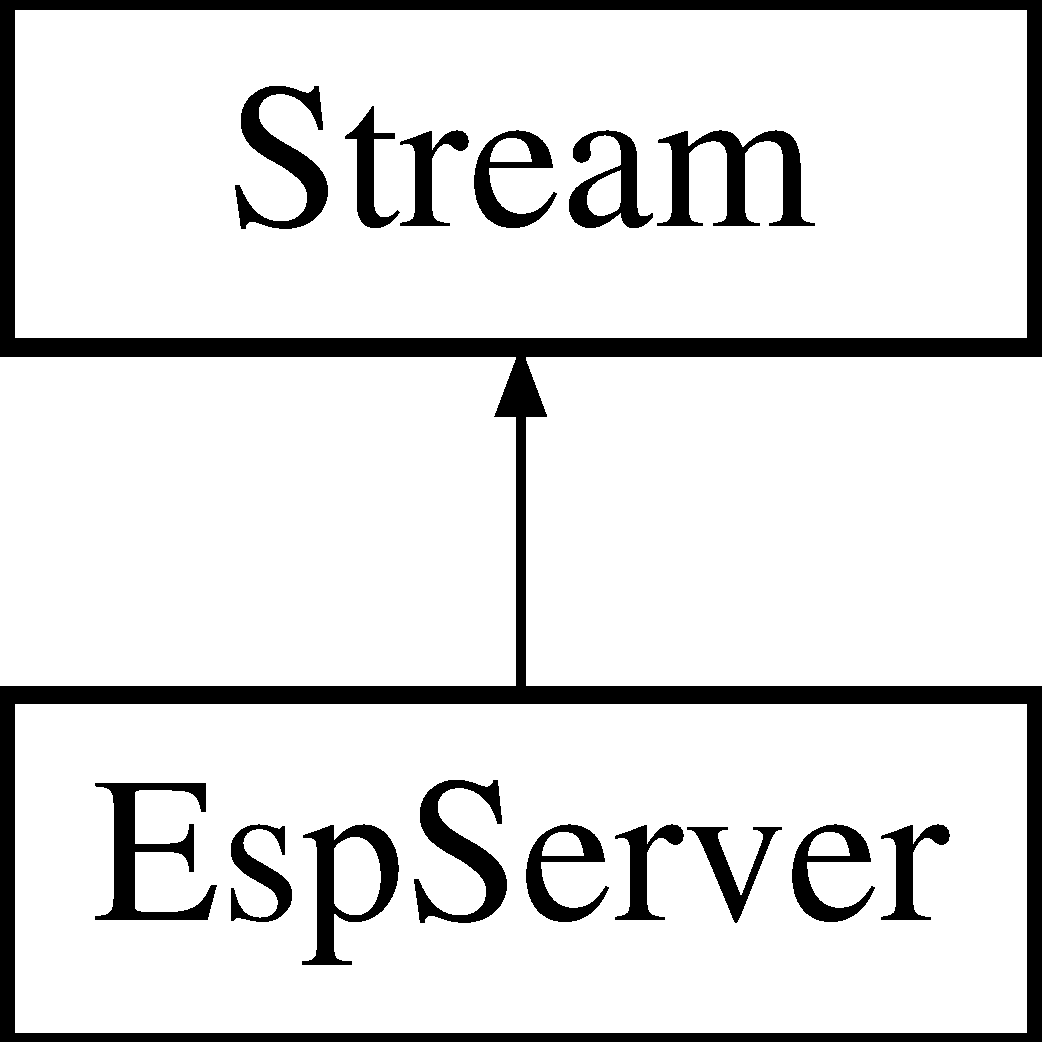
\includegraphics[height=2.000000cm]{class_esp_server}
\end{center}
\end{figure}
\subsection*{Public Member Functions}
\begin{DoxyCompactItemize}
\item 
\mbox{\Hypertarget{class_esp_server_a1d032e732d4733905d676ef016fcd43c}\label{class_esp_server_a1d032e732d4733905d676ef016fcd43c}} 
void {\bfseries begin} (Stream $\ast$esp\+\_\+serial, const char $\ast$ssid, const char $\ast$pass, uint16\+\_\+t port)
\item 
\mbox{\Hypertarget{class_esp_server_a55995fd6398892be5768da85dde4f533}\label{class_esp_server_a55995fd6398892be5768da85dde4f533}} 
void {\bfseries my\+\_\+ip} (char $\ast$buf, size\+\_\+t buflen)
\item 
\mbox{\Hypertarget{class_esp_server_a6a25e008ded89de0e4599df7170008fb}\label{class_esp_server_a6a25e008ded89de0e4599df7170008fb}} 
bool {\bfseries connected} ()
\item 
\mbox{\Hypertarget{class_esp_server_aad68b4972f6b8426004feeef6e98d02d}\label{class_esp_server_aad68b4972f6b8426004feeef6e98d02d}} 
virtual int {\bfseries available} ()
\item 
\mbox{\Hypertarget{class_esp_server_a005a9cd487f4ccb4ccef72197bf263b7}\label{class_esp_server_a005a9cd487f4ccb4ccef72197bf263b7}} 
virtual int {\bfseries peek} ()
\item 
\mbox{\Hypertarget{class_esp_server_ae47512714818b3b9a1d29d2bf1f70fdf}\label{class_esp_server_ae47512714818b3b9a1d29d2bf1f70fdf}} 
virtual int {\bfseries read} ()
\item 
\mbox{\Hypertarget{class_esp_server_a05062a3ac7c70a79e991b66789384bf1}\label{class_esp_server_a05062a3ac7c70a79e991b66789384bf1}} 
virtual void {\bfseries flush} ()
\item 
\mbox{\Hypertarget{class_esp_server_a0756c42343195dd1d1aa2f61c9b095bf}\label{class_esp_server_a0756c42343195dd1d1aa2f61c9b095bf}} 
virtual size\+\_\+t {\bfseries write} (const uint8\+\_\+t $\ast$buffer, size\+\_\+t size)
\item 
\mbox{\Hypertarget{class_esp_server_aecc7262ee265fd78affe24f35e49e1bb}\label{class_esp_server_aecc7262ee265fd78affe24f35e49e1bb}} 
size\+\_\+t {\bfseries write} (uint8\+\_\+t n)
\item 
\mbox{\Hypertarget{class_esp_server_ae3ba71ceb4df9357d8e258efe3e79f4d}\label{class_esp_server_ae3ba71ceb4df9357d8e258efe3e79f4d}} 
size\+\_\+t {\bfseries write} (unsigned long n)
\item 
\mbox{\Hypertarget{class_esp_server_ac256a11ccc8d32664729a7f5bfc71add}\label{class_esp_server_ac256a11ccc8d32664729a7f5bfc71add}} 
size\+\_\+t {\bfseries write} (long n)
\item 
\mbox{\Hypertarget{class_esp_server_afde7c57b12659422147d9a5e56b76148}\label{class_esp_server_afde7c57b12659422147d9a5e56b76148}} 
size\+\_\+t {\bfseries write} (unsigned int n)
\item 
\mbox{\Hypertarget{class_esp_server_a2a49890c886a2b0569b11e02f986f867}\label{class_esp_server_a2a49890c886a2b0569b11e02f986f867}} 
size\+\_\+t {\bfseries write} (int n)
\end{DoxyCompactItemize}


The documentation for this class was generated from the following files\+:\begin{DoxyCompactItemize}
\item 
Dumb\+Server.\+h\item 
Dumb\+Server.\+cpp\end{DoxyCompactItemize}

%--- End generated contents ---

% Index
\backmatter
\newpage
\phantomsection
\clearemptydoublepage
\addcontentsline{toc}{chapter}{Index}
\printindex

\end{document}
